% !TEX root = 0-main.tex
% !TEX encoding = UTF-8 Unicode
\chapter{Проектирование программного инструмента}
\label{cha:ch_2}

Прежде всего выделим сущности и определим действия, которые необходимы для решения задачи.

\begin{enumerate}
\item \textbf{Правильный шестиугольник} характеризуется весом и координатой расположения на гексагональной сетке. В качестве допустимых действий можно выделить: изменение веса, сравнение с другими подобными сущностями.
\item \textbf{Гексагональная сетка} характеризуется размерностью. Определяет правила для создания, управления, хранения гексов. 
\end{enumerate}
Для формирования данных о гексагональной сетке рассмотрим варианты: загрузка данных из файла, редактирование (как новой, так и загруженной) гексагональной сетки в графическом режиме.

\section{Системы координат}
Для работы с элементами гексагональной сетки необходима система координат. Источник \cite{red} описывает три системы координат для прямоугольного дискретного 
рабочего поля (\textit{ПДРП}). Определим эти три системы для РТДРП и добавим еще одну: 

\subsection{Координаты смещений}
 Данная система определяет смещение шестиугольника в сетке относительно точки отсчета. Возьмем за точку отсчета верхний левый угол полотна, на котором будет отрисовываться сетка (Рис. \ref{axis:offset}).

\subsection{Порядковые координаты}
\label{design:ordinal_axis}
Первый показатель зависит от порядкового номера среди остальных элементов на одном уровне, относительно левого края. Второй соответсвует уровню, на котором элемент расположен (Рис. \ref{axis:ordinal}).\par
В ПДРП координаты смещений являются индексом элемента массива, 
который характеризует шестиугольник с данными координатами. Но в РТДРП вершина находится в середине рабочего поля. Так что порядковые координаты будут определять индекс с данными о шестиугольнике в соответствующей структуре хранения. 

\begin{figure}[h]
\begin{center}
\begin{minipage}[h]{0.47\linewidth}
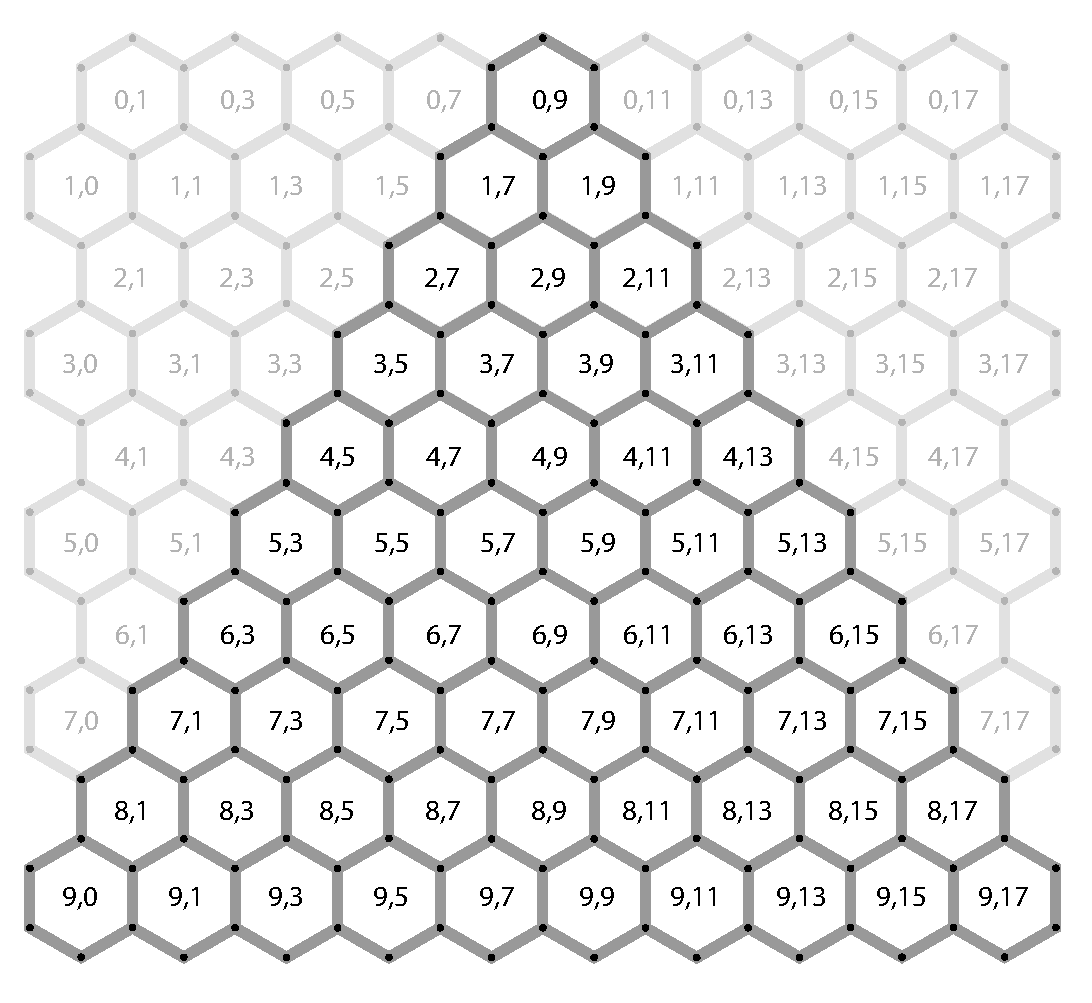
\includegraphics[width=1\linewidth]{inc/img/hexagon_offset}
\caption{Координаты смещений.} 
\label{axis:offset} 
\end{minipage}
\hfill 
\begin{minipage}[h]{0.47\linewidth}
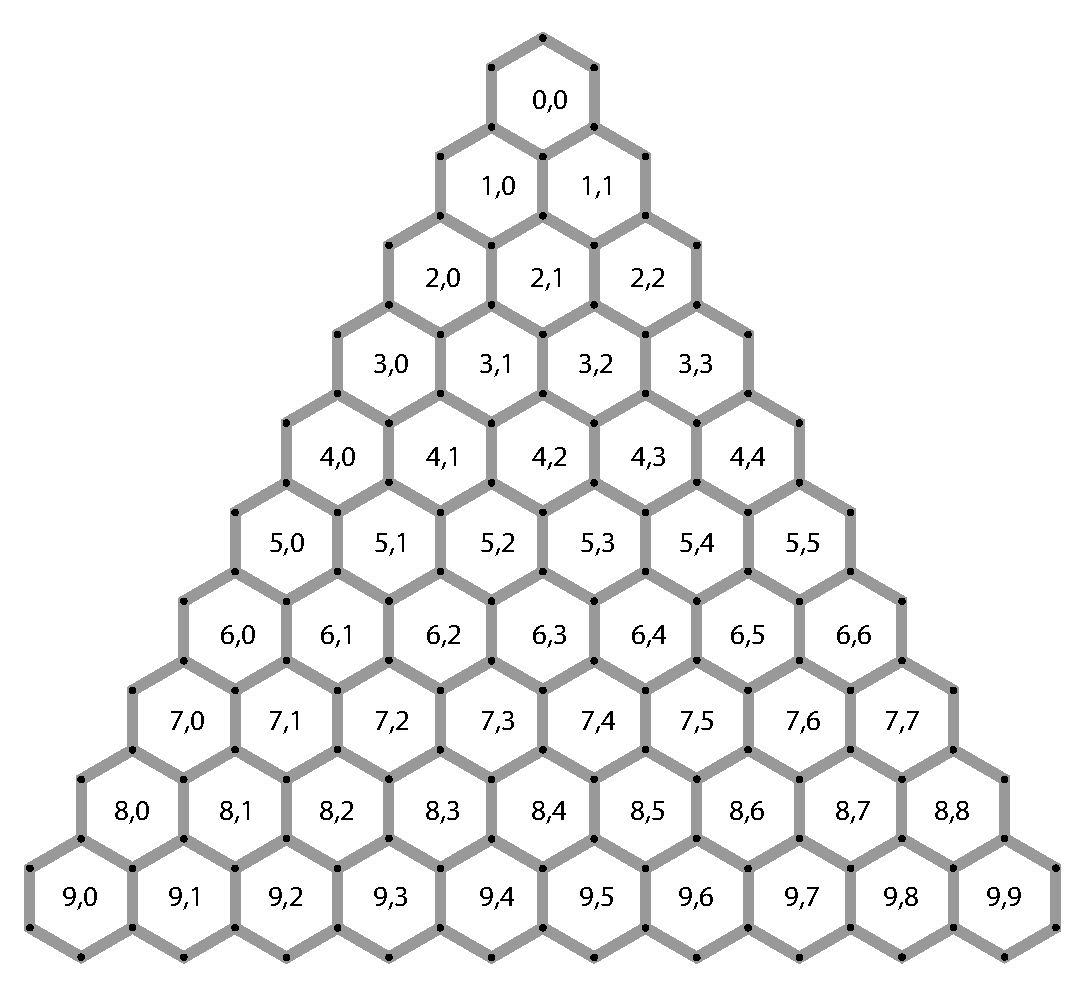
\includegraphics[width=1\linewidth]{inc/img/hexagon_ordinal}
\caption{Порядковые координаты.}
\label{axis:ordinal}
\end{minipage}
\end{center}
\end{figure}

\subsection{Кубические координаты}
Данная система имеет три оси координат \textit{X, Y, Z}. Согласно \cite{red}, берется сетка кубов в этой системе координат и из нее вырезается диагональная плоскость $x+y+z=0$. (Рис. \ref{axis:cube})

\par
Для вычисления центра системы координат относительно порядковой координаты, необходимо найти точку пересечения биссектрис равностороннего треугольника,  в который помещается гексагональная сетка.
$centerHexagon_{y} = 2\lfloor gridD / 3\rfloor $ --- ряд гексагональной сетки, где координата по оси $Z$ равна $0$.
$centerHexagon_{x} = centerR / 2 $ --- позиция шестиугольника в ряду $centerR$, у которого все координаты $0$.
\par Данная система удобна для различных арифметических действий с координатами элементов (можно воспользоваться стандартными операциями из декартовых координат: суммированием и вычитанием координат, умножением и делением на скалярную величину, а также расстояниями) и отлично подходит для работы с алгоритмами на графах.

\subsection{Осевые координаты}
Осевая система координат, иногда называемая «трапецеидальной», строится на основе двух или трёх координат из кубической системы координат. Поскольку у нас есть условие x + y + z = 0, третья координата не нужна. Осевые координаты полезны для хранения карт и отображения координат пользователю. Как и в случае с кубическими координатами, с ними можно использовать стандартные операции суммирования, вычитания, умножения и деления декартовых координат.\par
Преимущество этой системы перед сетками смещений в большей понятности алгоритмов. Недостатком системы является то, что хранение прямоугольной карты выполняется нелинейным способом. Некоторые алгоритмы ещё понятнее в кубических координатах, но поскольку есть условие $x + y + z = 0$, значит  можно вычислить третью подразумеваемую координату и использовать её в этих алгоритмах (Рис. \ref{axis:axial}).

\begin{figure}[h]
\begin{center}
\begin{minipage}[h]{0.47\linewidth}
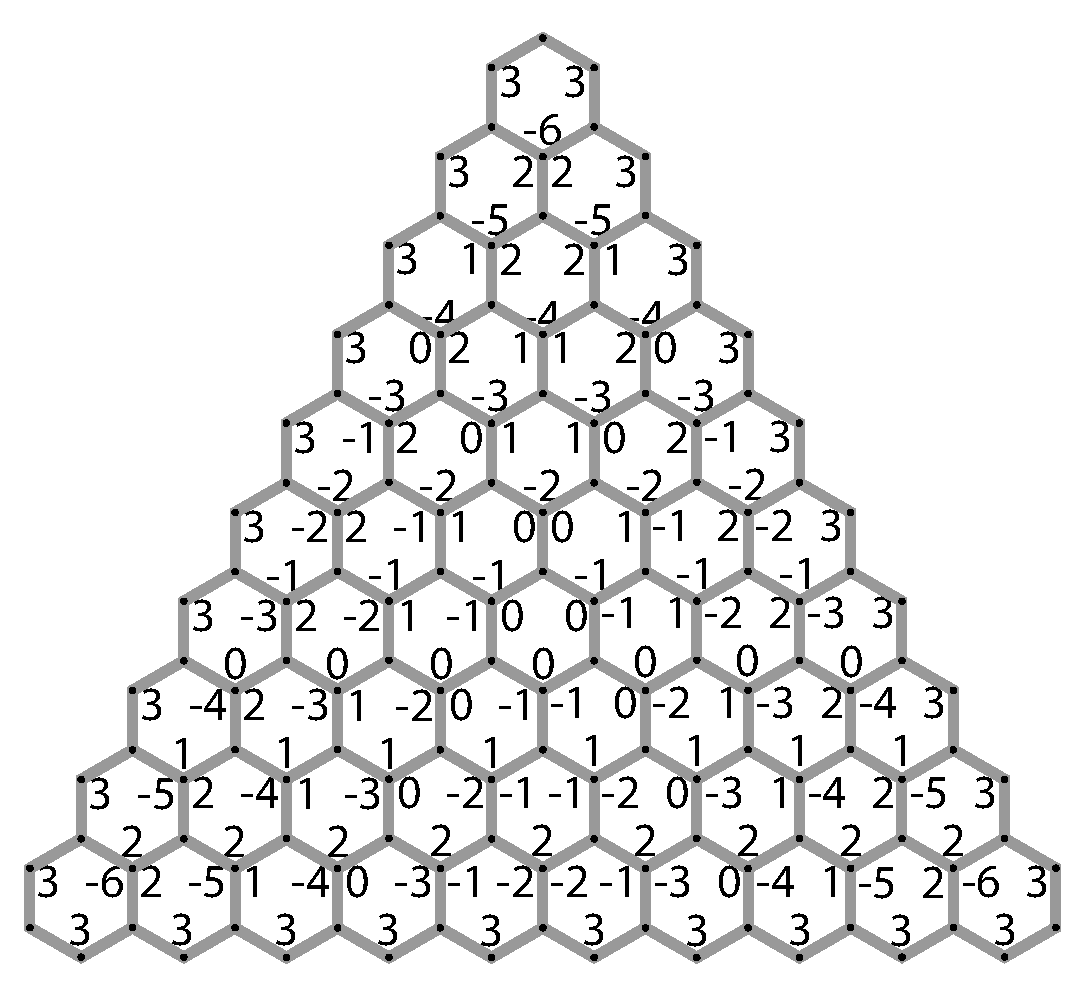
\includegraphics[width=1\linewidth]{inc/img/hexagon_cube}
\caption{Кубические координаты.} %% подпись к рисунку
\label{axis:cube} %% метка рисунка для ссылки на него
\end{minipage}
\hfill 
\begin{minipage}[h]{0.47\linewidth}
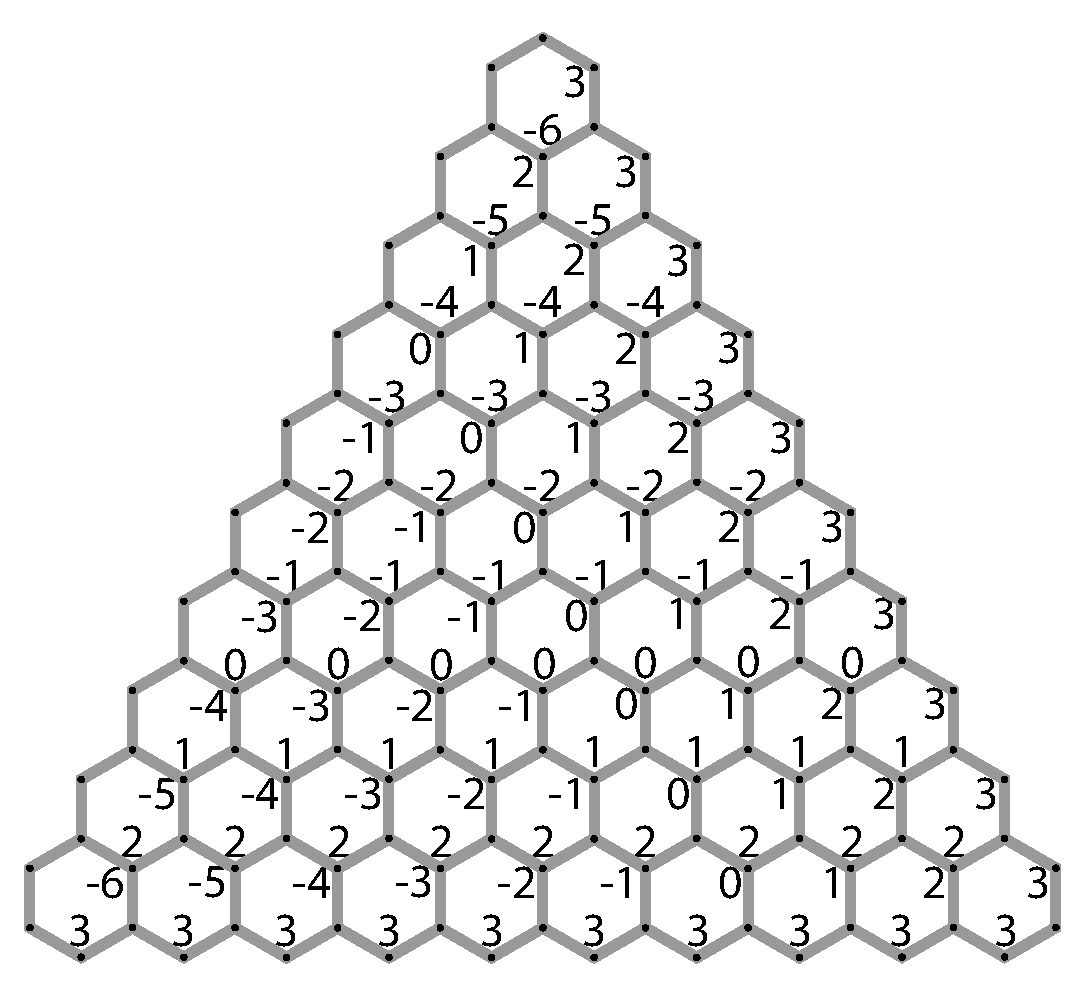
\includegraphics[width=1\linewidth]{inc/img/hexagon_axial}
\caption{Осевые координаты.}
\label{axis:axial}
\end{minipage}
\end{center}
\end{figure}

\section{Проектирование реализации алгоритма Дейкстры}
Данный алгоритм, согласно теории (раздел \ref{analysis:dijkstra}), работает со взвешенным орграфом. Пусть вершина --- это шестиугольник в орграфе, а вес дуги задается весом конечной вершины, так как это является водным условием задачи (Рис.\ref{hexagon:weight}).
\begin{figure}[h]
	\centering
	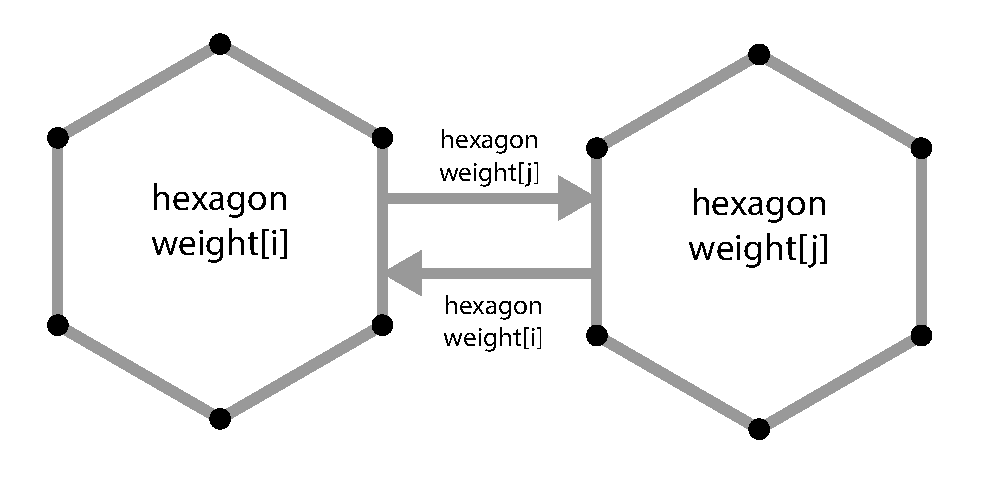
\includegraphics[height=0.3\textwidth]{inc/img/hexagon_weight}
	\caption{Определение веса шестиугольника.}
	\label{hexagon:weight}
\end{figure}
\par
Тогда, входными данными алгоритма является гексагональная сетка, начало и конец искомого пути.
\par Для упрощения структуры хранения гексагональной сетки можно ввести функцию нахождения соседних шестиугольников на основе кубических координат. Для этого необходимо вектор координат шестиугольника сложить поочередно с каждым из шести векторов $
\Bigg( 
\begin{bmatrix}-1\\1\\0\end{bmatrix},
\begin{bmatrix}1\\-1\\0\end{bmatrix},
\begin{bmatrix}0\\-1\\1\end{bmatrix},
\begin{bmatrix}0\\1\\-1\end{bmatrix},
\begin{bmatrix}1\\0\\-1\end{bmatrix}, 
\begin{bmatrix}-1\\0\\1\end{bmatrix}
\Bigg)
$вычисления соседа (Рис. \ref{hexagon:neighbors}), не забывая, что у элементов на границе РТДРП их количество равно или 4, или 2 (на вершинах РТДРП).   
\begin{figure}[h]
	\centering
	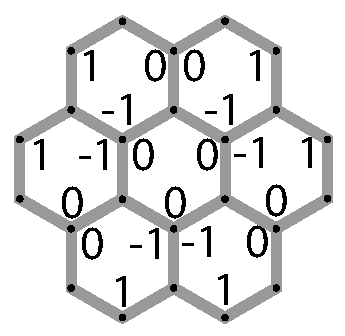
\includegraphics[height=0.3\textwidth]{inc/img/neib}
	\caption{Координаты для вычисления соседних шестиугольников.}
	\label{hexagon:neighbors}
\end{figure}
\par

\section{Проектирование графического интерфейса}
Консольное приложение реализуется в разы быстрее, чем с графическим интерфейсом. Относительно данной задачи неудобство консольного связано с вводом и выводом данных. При размерности РТДРП равной 100 будет необходимо ввести 5050 параметров каждого шестиугольника. А при правильном подходе к тестированию, возникнет необходимость в создании специализированных входных данных, которые позволят отследить работоспособность и правильность работы алгоритма. Редактирование такого количества данных потребует времени. А графический интерфейс позволит редактировать данные прямо на графическом представлении гексагональной сетки, что в разы сэкономит время и силы. Так же появляется возможность наглядно отслеживать работу алгоритма.
\par
Для этого необходимо разработать:
\begin{enumerate}
	\item Дизайн и логику главного окна;
	\item Отрисовку гексагональной сетки;
	\item Возможность взаимодействия с гексагональной сетки с помощью компьютерной мыши;
	\item Наглядное представление работы алгоритма Дейкстры.
\end{enumerate}
\subsection{Главное окно}
Необходимо предоставить возможность пользователю с помощью графического интерфейса создавать, открывать, редактировать и сохранять гексагональные сетки. А также воспроизводить алгоритм Дейкстры, отображать и сохранять его результат и промежуточные данные работы. Для этих задач необходимо в главном окне разместить соответсвующие кнопки для управления согласно ситуации. 
\subsection{Отрисовка гексагональной сетки}
\label{design:paint_hex_grid}
После запуска программы и инициирования создания новой или открытия сохраненной гексагональной сетки необходимо определиться с её размерами, чтобы РТДРП полностью помещалась в соотвествующий раздел главного окна. Согласно формулам \ref{hexGrid:gridHeight} и \ref{hexGrid:gridWidth} можно вычислить размер шестиугольника, взяв за $gridH$ высоту раздела или $gridW$ ширину раздела. Но для того, чтобы сетка точно поместилось, необходимо определить $min(gridH, gridW)$ и по соответствующей далее формуле (\ref{hexagon:sizeByGridHeight} или \ref{hexagon:sizeByGridWidth})  вычислить $hexagonSize$.
\begin{equation}
%\caption{Вычисление размера шестиугольника на основе ширины и высоты сетки.}
\label{hexagon:sizeByGridHeight}
hexagonSize = \frac{gridH}{2( \frac{3}{4}gridD+\frac{1}{4} )}
\end{equation}

\begin{equation}
%\caption{Вычисление размера шестиугольника на основе ширины и высоты сетки.}
\label{hexagon:sizeByGridWidth}
hexagonSize = \frac{gridW\sqrt{3}}{3\times gridD}
\end{equation}
Все необходимые данные для отрисовки гескагональной сетки собраны. Теперь необходимо описать шестиугольник, для его отрисовки. Согласно рисунку \ref{analysis:hexagonGridWithPoints}, зададим формулы для вычисления координаты в системе, где будет отображаться сетка. 
\par 
Из теории о координатах заметим, что на каждом ряду (уровне) сетки крайний левый шестиугольник начинает свое <<движение>> с середины (шестиугольник $(0,0)$ на Рис. \ref{axis:ordinal}) и до левой границы РТДРП (шестиугольник $(9,0)$ на Рис. \ref{axis:ordinal}). Воспользуемся данным замечанием и выведем формулу для этого элемента $leftHexagon_{level_{x}}$, это позволит воспользоваться логикой порядковых координат (раздел \ref{design:ordinal_axis}) и вычислять последующие элементы данного уровня.
\begin{equation}
%\caption{Вычисление размера шестиугольника на основе ширины и высоты сетки.}
\label{hex:leftHex}
leftHexagon_{level_{x}} = centerHexagon_{x} - \frac{r}{2}hexagonWidth
\end{equation}
Согласно вышеупомянутой теории и формулам, вычислим координаты точек, образующих шестиугольник.
\begin{figure}[h]
	\centering
	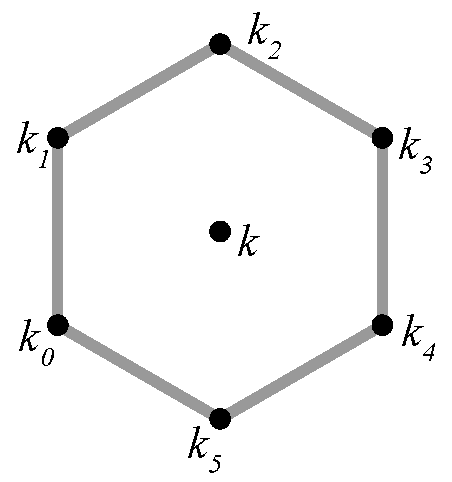
\includegraphics[width=0.25\linewidth]{inc/img/hexagon_edges}
	\caption{}
	\label{fig:}
\end{figure}


\begin{equation}
\begin{aligned}
&k \{leftHexagon_{level_{x}} + hexagonWidth\times currentHexagon_{level};  \\
&\hspace{3mm}\frac{1}{2} hexagonHeight +\frac{3}{4} hexagonHeight\times currentHexagon_{ordinal_{x}}\},  \\
&k_{0}\{k_{x}-\frac{1}{2}hexagonWidth; k_{y}+\frac{1}{4}hexagonHeight\},  \\
&k_{1}\{k_{x}-\frac{1}{2}hexagonWidth; k_{y}-\frac{1}{4}hexagonHeight\},  \\
&k_{2}\{k_{x};k_{y}-\frac{1}{2}hexagonHeight\},  \\
&k_{3}\{k_{x}+\frac{1}{2}hexagonWidth; k_{y}-\frac{1}{4}hexagonHeight\},  \\
&k_{4}\{k_{x}+\frac{1}{2}hexagonWidth; k_{y}+\frac{1}{4}hexagonHeight\},  \\
&k_{5}\{k_{x};k_{y}+\frac{1}{2}hexagonHeight\}.
\end{aligned}
%\phantom{\hspace{6cm}} %%<---adjust the value as you want
\end{equation}
Осталось назначить цвет каждому шестиугольнику. Весьма логично связать гексагональную сетку с <<трудно проходимым лесом>>, в котором вес шестиугольника --- <<стоимость>> или <<сложность>> прохождения данного участка.

\begin{figure}[h]
\begin{center}
\begin{minipage}[h]{0.47\linewidth}
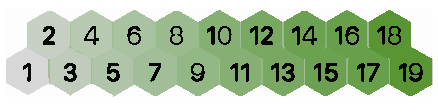
\includegraphics[width=1\linewidth]{inc/img/hexagon_gradient}
\caption{Пример раскраски гексагональной сетки.} %% подпись к рисунку
\label{axis:cube} %% метка рисунка для ссылки на него
\end{minipage}
\hfill 
\begin{minipage}[h]{0.47\linewidth}

\includegraphics[width=1\linewidth]{inc/img/gradient}
\caption{Цветовой градиент раскраски шестиугольника.}
\label{axis:axial}
\end{minipage}
\end{center}
\end{figure}

Для \textbf{создания svg файла} будут использоваться аналогичные методики и формулы.
\subsection{Взаимодействия с гексагональной сетки}

Взаимодействие будет происходить с помощью компьютерной мыши. Можно выделить несколько способов определения нужного шестиугольника и один из самых простых --- это перебор и сравнение координат нажатия относительно координат вершин шестиугольников, но это нерационально, особенно при больших размерах. Другой --- конвертировать координату нажатия относительно осевых координат. Для этого необходимо:
\begin{enumerate}
	\item Сместить систему координат мыши относительно центра осевой системы координат. В результате, координаты нажатия изменятся относительно смещения;
	\item Далее, необходимо сделать поворот осей мыши на 60\degree. То есть, вектор координат умножаем на матрицу поворота $\begin{bmatrix}\sqrt{3}/3& -1/3\\0& 2/3\end{bmatrix}$;
	\item В заключении, осуществим целочисленное деление (без округления) координат на $2\times hexagonSize$. 
\end{enumerate}
%TODO Вставить изображения
\begin{figure}[h]
\begin{center}
\begin{minipage}[h]{0.47\linewidth}
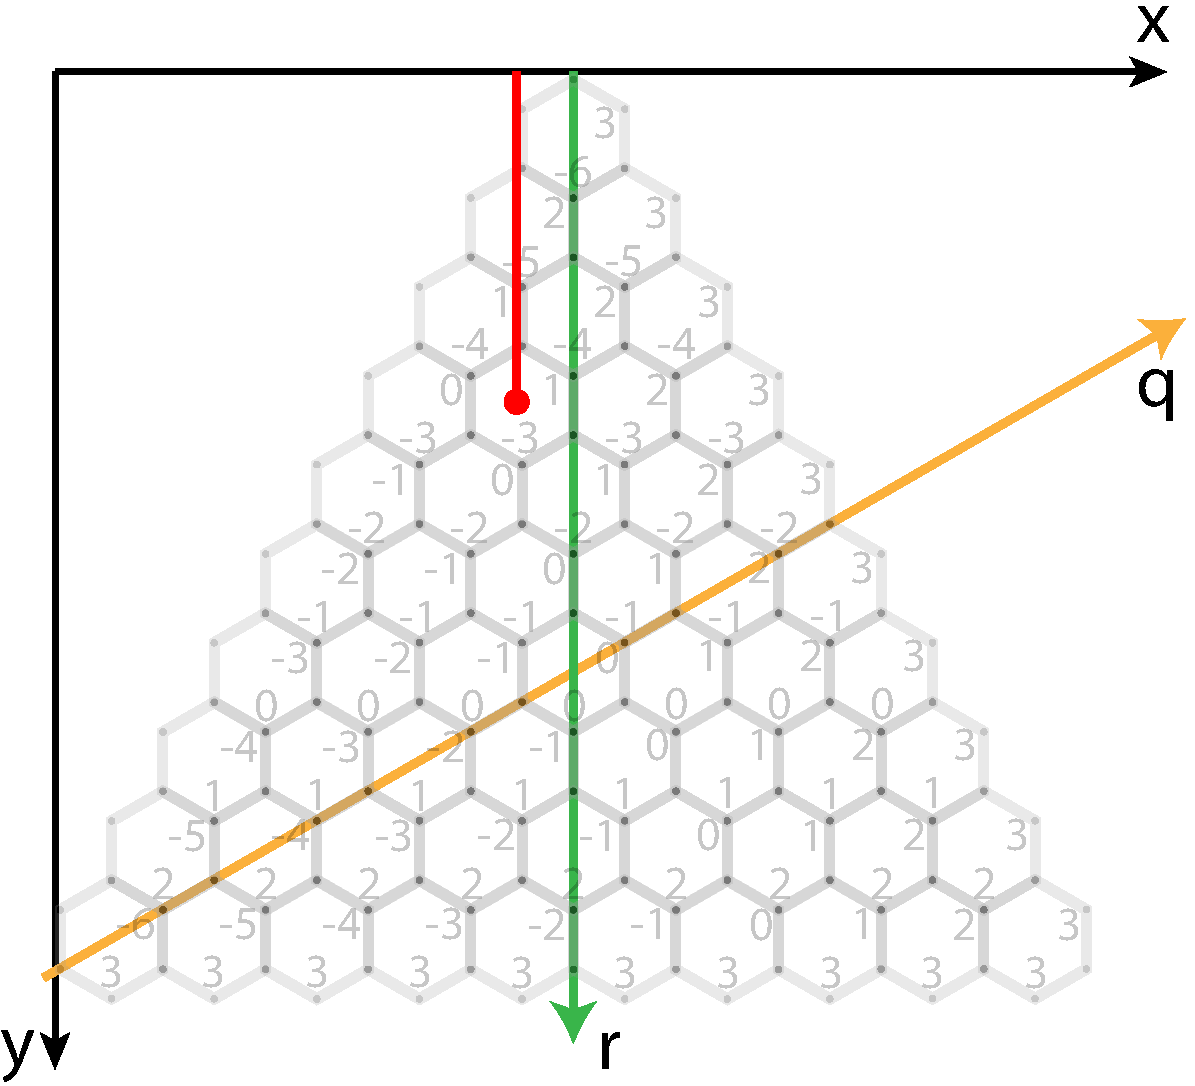
\includegraphics[width=1\linewidth]{inc/img/calcPoint_two}
\caption{Проекция координаты нажатия на ось $X$.} %% подпись к рисунку
\label{axis:cube} %% метка рисунка для ссылки на него
\end{minipage}
\hfill 
\begin{minipage}[h]{0.47\linewidth}
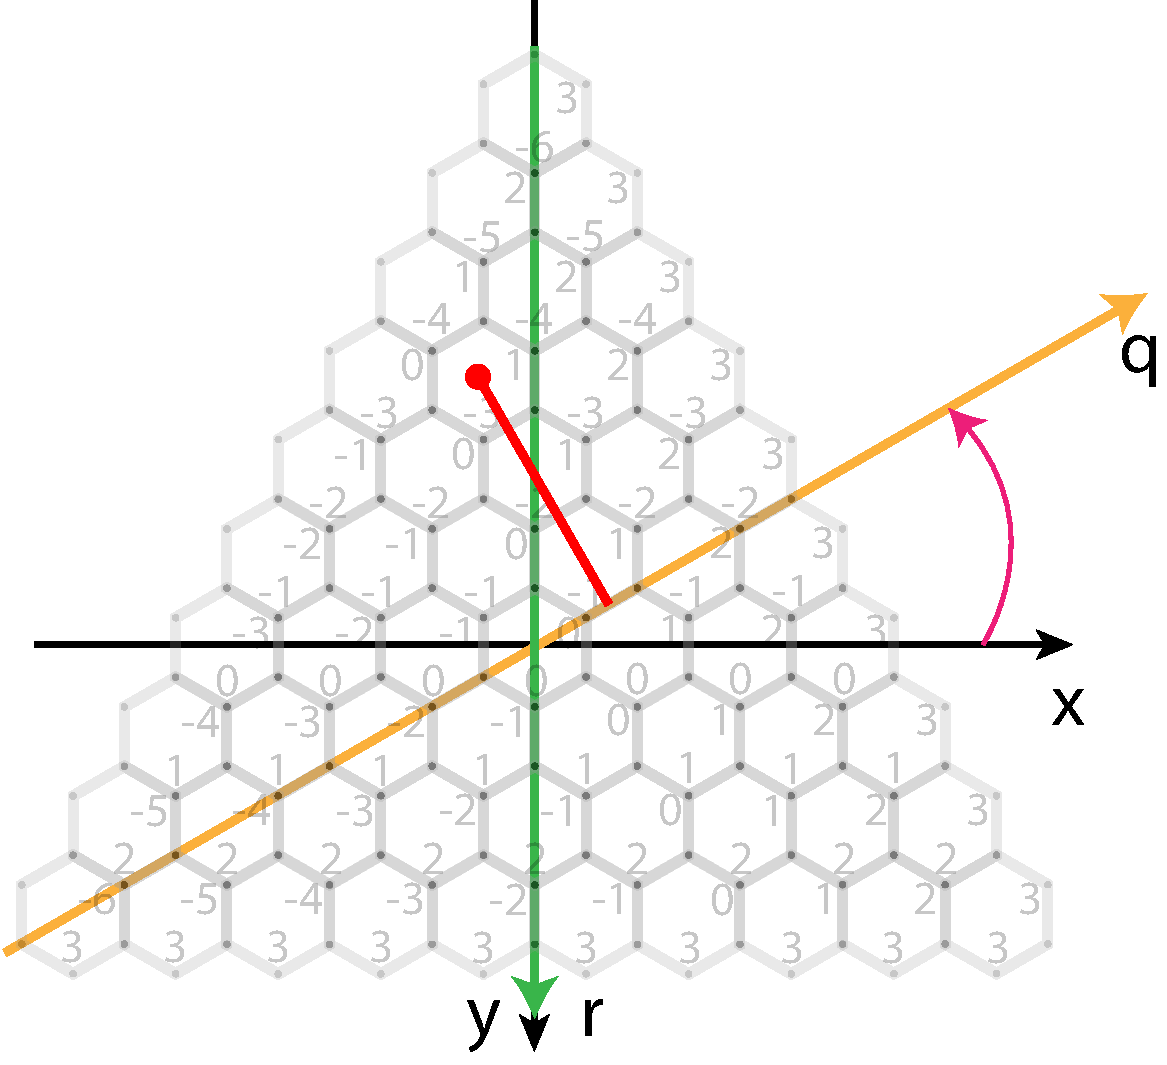
\includegraphics[width=1\linewidth]{inc/img/calcPoint_three}
\caption{Проекция координаты нажатия на ось $Q$.}
\label{axis:axial}
\end{minipage}
\end{center}
\end{figure}

\subsection{Проектирование вывода результата работы алгоритма Дейкстры}
Согласно теории (раздел \ref{analysis:dijkstra}), результатом работы алгоритма является вектор с длинами кратчайших путей из начала до всех остальных вершин. Следовательно, в качестве результата и промежуточного результата работы алгоритма целесообразно брать этот вектор и в качестве веса шестиугольника отображать длину (стоимость, сложность) кратчайшего пути до него.